\tikzset{every picture/.style={line width=0.75pt}} %set default line width to 0.75pt        

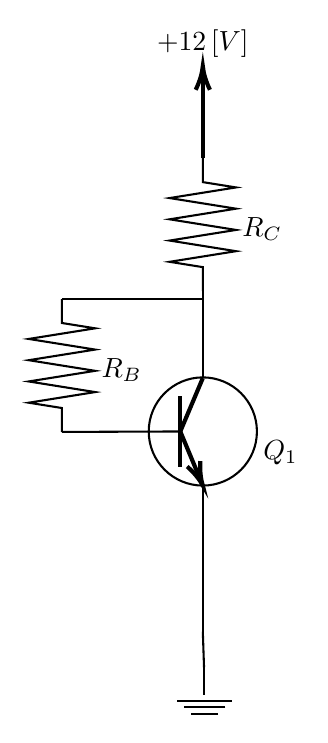
\begin{tikzpicture}[x=0.75pt,y=0.75pt,yscale=-.8,xscale=.8]
%uncomment if require: \path (0,445); %set diagram left start at 0, and has height of 445

%Shape: Resistor [id:dp576364330099814] 
\draw   (295.42,176.29) -- (295.42,190.69) -- (315.42,193.89) -- (275.42,200.29) -- (315.42,206.69) -- (275.42,213.09) -- (315.42,219.49) -- (275.42,225.89) -- (315.42,232.29) -- (275.42,238.69) -- (295.42,241.89) -- (295.42,256.29) ;
%Straight Lines [id:da8771969312931523] 
\draw    (295.42,176.29) -- (337.85,176.29) ;
%Straight Lines [id:da41124917033766106] 
\draw    (337.85,176.29) -- (380.27,176.29) ;
%Shape: Resistor [id:dp32430912394809286] 
\draw   (380.27,91.44) -- (380.27,105.84) -- (400.27,109.04) -- (360.27,115.44) -- (400.27,121.84) -- (360.27,128.24) -- (400.27,134.64) -- (360.27,141.04) -- (400.27,147.44) -- (360.27,153.84) -- (380.27,157.04) -- (380.27,171.44) ;
%Straight Lines [id:da16395222634879947] 
\draw    (366.7,256.01) -- (295.42,256.29) ;
%Shape: Circle [id:dp09876127689341485] 
\draw   (347.7,256.01) .. controls (347.7,238.02) and (362.28,223.44) .. (380.27,223.44) .. controls (398.27,223.44) and (412.85,238.02) .. (412.85,256.01) .. controls (412.85,274) and (398.27,288.59) .. (380.27,288.59) .. controls (362.28,288.59) and (347.7,274) .. (347.7,256.01) -- cycle ;
%Straight Lines [id:da7855487082641662] 
\draw [line width=1.5]    (366.7,277.23) -- (366.7,234.8) ;
%Straight Lines [id:da6420856407737783] 
\draw    (380.27,223.86) -- (380.27,171.44) ;
%Straight Lines [id:da9346216852859565] 
\draw [line width=1.5]    (366.7,256.01) -- (379.12,285.82) ;
\draw [shift={(380.27,288.59)}, rotate = 247.38] [color={rgb, 255:red, 0; green, 0; blue, 0 }  ][line width=1.5]    (14.21,-4.28) .. controls (9.04,-1.82) and (4.3,-0.39) .. (0,0) .. controls (4.3,0.39) and (9.04,1.82) .. (14.21,4.28)   ;
%Straight Lines [id:da5297912314249998] 
\draw    (381,398) -- (380.27,376.59) ;
%Straight Lines [id:da006223218346351644] 
\draw [line width=1.5]    (366.7,256.01) -- (380.27,223.86) ;
%Straight Lines [id:da9701929454236062] 
\draw    (380.27,376.59) -- (380.27,288.59) ;
%Straight Lines [id:da13224312413179473] 
\draw    (381,398) -- (381,414.42) ;
%Straight Lines [id:da10473520328776764] 
\draw    (397.84,418.13) -- (381.42,418.13) ;
%Straight Lines [id:da46427341450112913] 
\draw    (381.42,418.13) -- (365,418.13) ;
%Straight Lines [id:da9976365744338328] 
\draw    (389.42,426.13) -- (373,426.13) ;
%Straight Lines [id:da39363951353981896] 
\draw    (381.42,422.13) -- (369,422.13) ;
%Straight Lines [id:da2887972782852376] 
\draw    (393.84,422.13) -- (381.42,422.13) ;
%Straight Lines [id:da30358936692439087] 
\draw [line width=1.5]    (380.27,91.44) -- (380.27,39.02) ;
\draw [shift={(380.27,36.02)}, rotate = 90] [color={rgb, 255:red, 0; green, 0; blue, 0 }  ][line width=1.5]    (14.21,-4.28) .. controls (9.04,-1.82) and (4.3,-0.39) .. (0,0) .. controls (4.3,0.39) and (9.04,1.82) .. (14.21,4.28)   ;

% Text Node
\draw (317.42,210.09) node [anchor=north west][inner sep=0.75pt]    {$R_{B}$};
% Text Node
\draw (402.27,125.24) node [anchor=north west][inner sep=0.75pt]    {$R_{C}$};
% Text Node
\draw (380.27,32.62) node [anchor=south] [inner sep=0.75pt]    {$+12\left[\text{V}\right]$};
% Text Node
\draw (414.85,259.41) node [anchor=north west][inner sep=0.75pt]    {$Q_{1}$};


\end{tikzpicture}
